\chapter{Vulnerability overview}
Table \ref{tbl:vuln overview} depicts all vulnerabilities found during the penetration test. They are categorized by their risk and potential and are differentiated in the categories low, medium, high and critical. 
We are grouping the vulnerabilities by their CVSS score the following way:

\begin{table}[h]
	\centering
	\begin{tabular}{| p{3cm} | p{5cm} |}
		\hline 
		CVSS score & Category\\
		\hline 
		9.0 - 10.0 & \cellcolor{codepurple}Critical\\
		\hline 
		7.0 - 8.9 & \cellcolor{red}High\\
		\hline 
		4.0 - 6.9 & \cellcolor{orange}Medium\\
		\hline
		0.1 - 3.9 & \cellcolor{yellow}Low\\
		\hline
	\end{tabular}
	\caption{Grouping}
	\label{tbl:grouping}
\end{table}

Figure shows the overview of vulnerabilities grouped by asset.

\begin{figure}[h]
\centering
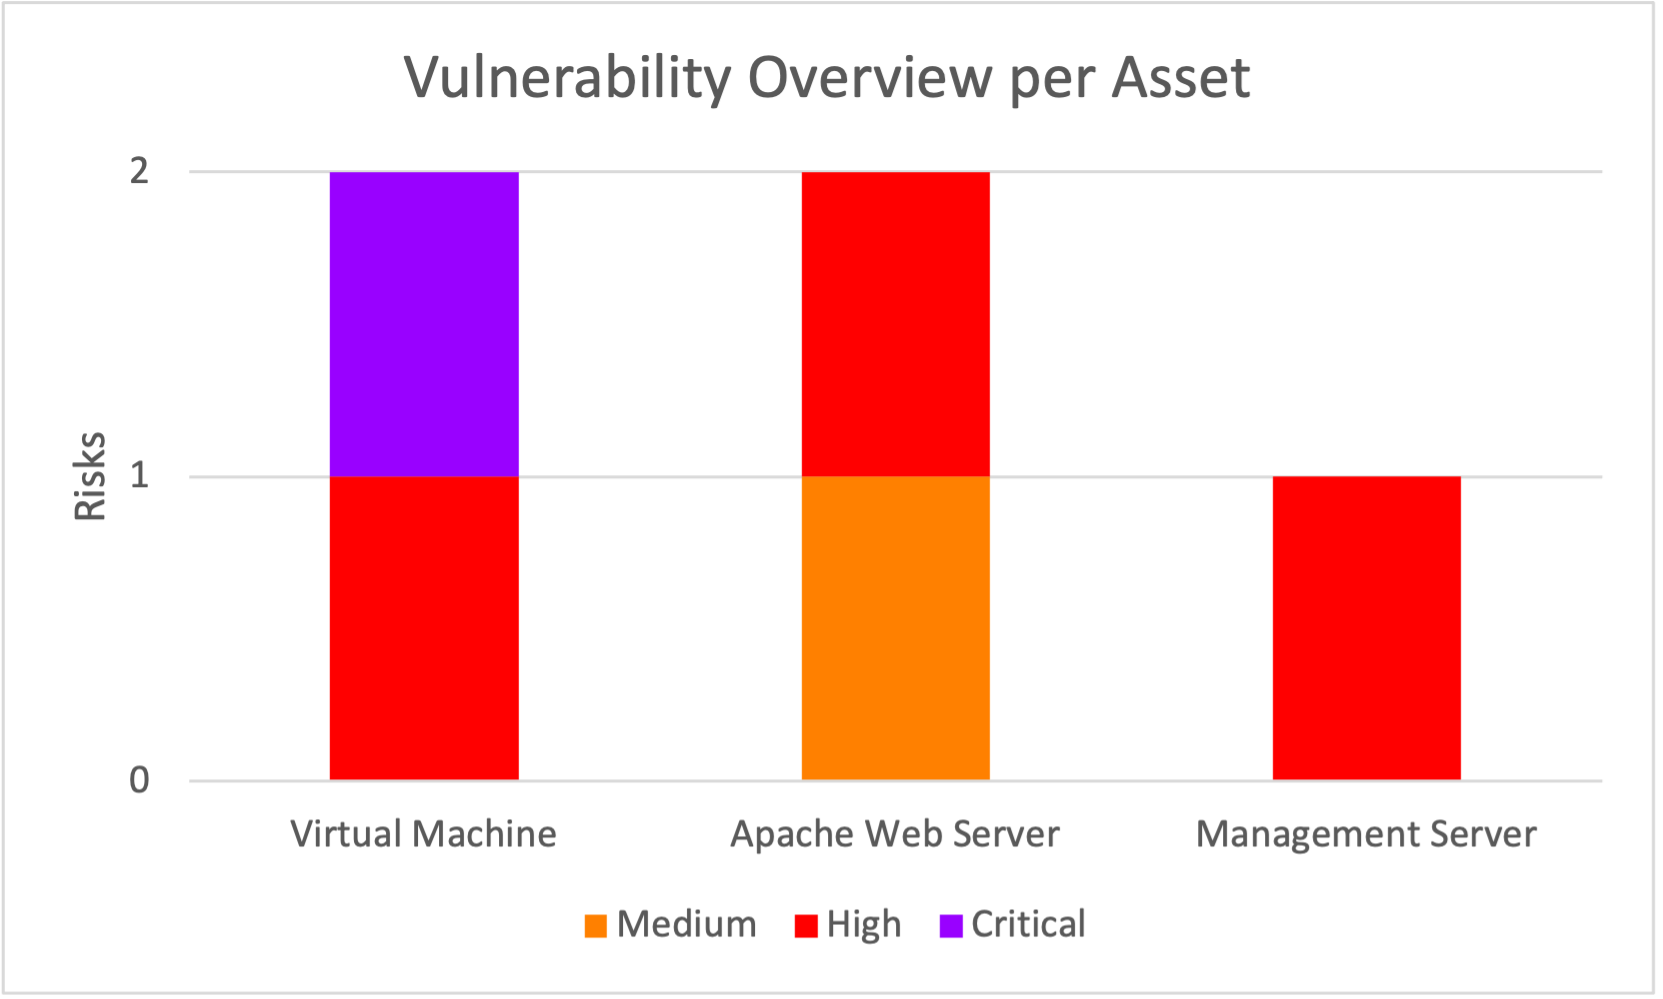
\includegraphics[width=\textwidth]{img/vuln_chart.png}
\caption{Vulnerability Overview}
\end{figure}

\begin{table}[h]
	\begin{tabular}{| l | l | p{7cm} | l | l |}
		\hline 
		Risk & Asset & Vulnerability & Section & Page\\
		\hline 
		\cellcolor{codepurple}Critical & Virtual Machine & Weak Password &  \ref{weak_password} & \pageref{weak_password} \\
		\hline 
		\cellcolor{red}High & Virtual Machine & Privilege Escalation &  \ref{privilege_escalation}& \pageref{privilege_escalation}\\
		\hline 
		\cellcolor{red}High & Apache Web Server & Outdated Version &  \ref{outdated_version} & \pageref{outdated_version} \\
		\hline 
		\cellcolor{orange}Medium & Apache Web Server & Information Disclosure & \ref{information_disclosure} & \pageref{information_disclosure} \\
		\hline
		\cellcolor{red}High & Management Server & Broken Authentication & \ref{management_server} & \pageref{management_server}\\
		\hline 
	\end{tabular}
	\caption{Vulnerability Overview}
	\label{tbl:vuln overview}
\end{table}